%!TEX root = widefieldscan.tex
\svnidlong
{$HeadURL$}
{$LastChangedDate$}
{$LastChangedRevision$}
{$LastChangedBy$}

\ifhtml
\else
\begin{center}
	\fbox{
		\begin{minipage}{.618\columnwidth}
		The section below is versioned at \url{\svnkw{HeadURL}} (last commit @ \svnfileday.\svnfilemonth.\svnfileyear \space \svnfilehour:\svnfileminute, Revision: \svnkw{LastChangedRevision}).
		\end{minipage}
	} 
\end{center}
\fi

\section{Materials and Methods}
\label{sec:materials and methods}
\cbstart
\subsection{Sample Preparation and Image Acquisition}
To test the enhancement of the FOV of the tomographic microscopy, we used rat lung samples, prepared according to~\citet{Schittny1997,Schittny1998}\todo{citations (taken from Schittny2008) still valid for our protocol?}. Briefly, lungs of Sprague-Dawley rats have been extracted after they have been perfused and filled with phosphate buffered saline by instillation via tracheotomy until the mid respiratory lung volume was reached. Handling of the animals before and during the experiments, as well as the experiments themselves, were approved and supervised by the Swiss Agency for the Environment, Forests and Landscape and the Veterinary Service of the Canton of Bern.

The extracted lung lobes have been fixed in \SI{2.5}{\percent} glutaraldehyde (C$_5$H$_8$O$_2$). For the preparation of the imaging the samples have been postfixed---comparable to electron microscopy protocols---with \SI{1}{\percent} osmium tetroxide (OsO$_4$) and stained with \SI{4}{\percent} uranyl acetate (C$_4$H$_6$O$_6$U), dehydrated in a graded series of ethanol and transferred into paraffin. The lung samples have been mounted onto standard electron microscopy sample mounts with a diameter of approximately \SI{13}{\milli\meter} (PLANO GmbH, Wetzlar, Germany) using paraffin.
\cbend

\subsection{SRXTM}
All experiments were performed at the TOMCAT beamline, Swiss Light Source, Paul Scherrer Institut, Villigen, Switzerland. %; , which is located at the X02DA port of the SLS and is one of 17 currently operating beamlines.
TOMCAT receives photons from a \SI{2.9}{\tesla} super-bending magnet. The critical energy of this super-bending magnet is \SI{11.1}{\kilo\electronvolt} (corresponding to a wavelength of \SI{1.22}{\angstrom}). A double crystal multilayer monochromator covers an energy range between 6 and \SI{45}{\kilo\electronvolt} with a bandwidth range of a few percent to a few per mille. Detailed technical specifications of the beamline and beam characteristics have been described by~\citet{Stampanoni2006a,Stampanoni2007}.

\subsubsection{Image Acquisition}
\label{seq:Image Acquisition}
The sample holder at TOMCAT is equipped with an appropriate collet chuck to mount standard electron microscopy (EM) sample tables into the beam. The samples have been scanned at an x-ray energy of \SI{12.6}{\kilo\electronvolt}. After penetration of the sample, the x-rays are converted into visible light by a Ce-doped YAG scintillator (Crismatec Saint-Gobain, Nemours, France). The projection images were further magnified by diffraction limited microscope optics and digitized by a high-resolution 2048\(\times\)2048 pixel CCD camera (pco.2000, PCO AG, Kelheim, Germany) with 14 bit dynamic range.% which can record projections into the internal memory of \SI{4}{\giga\byte}.
The lung samples were imaged using a 10\(\times\) magnification, with 2\(\times\)2 binning and \SI{125}{\milli\second} exposure time or no binning and \SI{500}{\milli\second} exposure time, resulting in isotropic voxels with a side length of \SI{1.48}{\micro\meter} or \SI{0.74}{\micro\meter}, respectively\todo{for B--T what is it exactly, what is it for Sophies Sample? -> be precise!}.

\subsubsection{Generation of tomographic datasets}
The principles of x-ray computed tomography are explained by \citet{Kak2002}. Briefly, projection images $I_{Pr}$---essentially single radiographies---of the sample are recorded at several angular positions between \SI{0}{\degree} and \SI{180}{\degree}. Additionally, a set of dark ($I_{D}$) and flat images ($I_{F}$) are recorded. The dark image set is obtained with a closed shutter at the start of the scan, it captures the camera noise and dark current and is used to baseline correct the projection images. The flat image set is recorded at the start and at the end of the scan, it captures the beam profile and is used to normalize the projection images. The corrected projection images $I_{cPr}$ are obtained by correcting $I_{Pr}$ with the average dark ($\overline{I_{D}}$) and average flat image ($\overline{I_{F}}$) using equation~\ref{eq:cpr}.
\begin{equation}
	I_{cPr} = -ln\left(\frac{I_{Pr}-\overline{I_{D}}}{\overline{I_{F}}-\overline{I_{D}}}\right)
	        = ln(\overline{I_{F}}-\overline{I_{D}})-ln(I_{Pr}-\overline{I_{D}})
	\label{eq:cpr}
\end{equation}
The corrected projections are then transformed into so-called sinograms, where the $n$\textsuperscript{th} is composed of the $n$\textsuperscript{th} line of every corrected projection. One sinogram thus contains as many rows as the amount of obtained corrected projections---the angular steps---and as many columns as the width of the projection images. Each sinogram corresponds to one slice of the tomographic dataset. The $n$\textsuperscript{th} slice of the tomographic scan can be reconstructed from the $n$\textsuperscript{th} sinogram using a standard filtered back-projection~\cite{Kak2002,Hsieh2003} or gridrec~\cite{Dowd1999} algorithm. The absorption properties of the sample are encoded by the gray values of the reconstructed dataset. The full work flow from image acquisition to tomographic dataset on the disk contains several steps more, detailed explanations are described by~\citet{Hintermueller2009}.

%\subsection{Image Processing}
%\label{subsec:image processing}
%After the acquisition of the sub-scan projection images, these image sets are corrected with the so called dark field and flat field images. The dark field images are obtained while all the shutters are closed---thus no x-rays are present---and are used for the detection of camera noise and dark current. The flat field images (FI) are obtained with x-ray beam, but without the sample. They are recorded to remove the varying beam profile brightness from the projection images. The projections (PI) are first baseline corrected, then the average of the dark images is subtracted and afterwards they are normalized into corrected projections (CPR) as seen in equation~\ref{eq:correction}:%
% \begin{equation}
%	\text{CPR}=-ln\left(\frac{\text{PI}}{\text{FI}}\right)=ln(\text{FI})-ln(\text{PI})
%	\label{eq:correction}
% \end{equation}
\subsubsection{Covering a broad FOV}
\label{subsec:covering a broad fov}
For parallel beam geometry, tomographic images are obtained by rotating the sample over \SI{180}{\degree} and acquiring images equidistantly between \SI{0}{\degree} and \SI{180}{\degree}, as shown in figure~\ref{subfig:scanning-possibilities}. After reconstruction the width of the image corresponds to the FOV of the camera.

If the sample to be imaged is larger than the available FOV, a \SI{360}{\degree}-scan is performed. Projections are obtained over a full rotation of the sample, while the sample is positioned in front of the camera in such a way that it only covers half the FOV of the detector. After acquisition of the projection images, half of the dataset has to be flipped and the projections at position $P_{x}$ and $P_{x+\SI{180}{\degree}}$ are stitched together to projection images covering two times the FOV of the camera.

\begin{figure*}
	\noindent\makebox[\textwidth]{%
		\subfloat[Three different scanning configurations for increasing sample diameter.]{%
			%\documentclass{article}
%\usepackage[demo]{graphicx}
%\usepackage{subfig}
%\usepackage{tikz}
%	\usetikzlibrary{patterns}
%\usepackage{multirow}
%\usepackage{siunitx}
%\begin{document}
%\begin{figure}
%\centering
%%%%%%%%%%%%%%%%%%%%%%%%%%%%%
\begin{tikzpicture}
	%%%%%%%%%%%%%%%%%%%
	%      grid       %
	%%%%%%%%%%%%%%%%%%%
%		\def\stop{10}
%		\draw [color=gray] (0,0) grid (\stop,\stop);
%		\draw [shade] (0,0) circle (0.25) node {origin};
%		\draw [shade] (\stop,\stop) circle (0.25) node {\stop,\stop};
	%%%%%%%%%%%%%%%%%%%
	%       180       %
	%%%%%%%%%%%%%%%%%%%
		\def\startAtY{9}
		\def\BeamLength{4}
		\def\length{2}
		\node [anchor=north] at (0.5,\startAtY) {a)};
		%camera
			\draw [fill=gray] (0,\startAtY) rectangle (1,\startAtY+1);
			\node [anchor=center] at (0.5,\startAtY+1+.25) {camera};
		% beam
			% inner rays
			\foreach \x in {9,9.1,...,10}
				\draw[gray!50,<-] (1,\x) -- (\BeamLength+1,\x);
			% outer rays
			\foreach \x in {0,1}
				\draw[<-] (1,\startAtY+\x) -- (\BeamLength+1,\startAtY+\x);
			% label				
			\node at (\BeamLength+0.5,\startAtY+1+.25) {beam};
		%sample
			\fill [color=gray,nearly transparent] (0.5*\BeamLength+1,\startAtY+0.5) circle (0.5);
			\fill (0.5*\BeamLength+1,\startAtY+0.5) circle (0.025);
			\draw [thick] (0.5*\BeamLength+1,\startAtY+0.5) circle (0.5);
			\draw [thick,->] (0.5*\BeamLength+1,\startAtY+0.25)   arc (-90:90:0.25);
			\node at (0.5*\BeamLength+1,\startAtY+1+0.25) {sample};
	%%%%%%%%%%%%%%%%%%%
	%       360       %
	%%%%%%%%%%%%%%%%%%%
		\def\startAtY{6}
		\node [anchor=north] at (0.5,\startAtY) {b)};
		%camera
			\draw [fill=gray] (0,\startAtY) rectangle (1,\startAtY+1);
%			\node at (0.5,\startAtY-.25) {camera};
		% beam
			% inner rays
			\foreach \x in {6,6.1,...,7}
				\draw[gray!50,<-] (1,\x) -- (\BeamLength+1,\x);
			% outer rays
			\foreach \x in {0,1}
				\draw[<-] (1,\startAtY+\x) -- (\BeamLength+1,\startAtY+\x);
			% label				
%			\node at (\BeamLength+0.5,\startAtY+1.25) {beam};
		%sample
			\fill [color=gray,nearly transparent] (0.5*\BeamLength+1,\startAtY+1) circle (1);
			\fill (0.5*\BeamLength+1,\startAtY+1) circle (0.025);
			\draw [thick] (0.5*\BeamLength+1,\startAtY+1) circle (1);
			\draw [thick,->] (0.5*\BeamLength+1,\startAtY+0.75) arc (-85:265:0.25);
%			\node at (0.5*\BeamLength+1,\startAtY-0.75) {sample};
	%%%%%%%%%%%%%%%%%%%
	% Wide Field Scan %
	%%%%%%%%%%%%%%%%%%%
		\def\startAtY{2}
		\node [anchor=north] at (0.5,\startAtY) {c)};
		%camera
			\draw [fill=gray] (0,\startAtY) rectangle (1,\startAtY+1);
%			\node at (0.5,\startAtY-.25) {camera};
		% beam
			% inner rays
			\foreach \x in {2,2.1,...,3}
				\draw[gray!50,<-] (1,\x) -- (\BeamLength+1,\x);
			% outer rays
			\foreach \x in {0,1}
				\draw[<-] (1,\startAtY+\x) -- (\BeamLength+1,\startAtY+\x);
			% label				
%			\node at (\BeamLength+0.5,\startAtY+1.25) {beam};
		% shaded samples
		\foreach \y/\position/\color in {\startAtY-0.5/1/red,\startAtY+0.5/2/green,\startAtY+1.5/3/blue}
			{
				\fill [color=\color, nearly transparent] (0.5*\BeamLength+1,\y) circle (1.5);
			}
		\pattern [pattern=checkerboard light gray] (0.5*\BeamLength+1,3) arc (90:-90:1.5) -- ++(0,1) arc (-90:90:0.5);
		\fill [color=red, semitransparent]   (0.5*\BeamLength+1,3) arc (90:-90:1.5) -- ++(0,1) arc (-90:90:0.5);
		\pattern [pattern=horizontal lines gray] (0.5*\BeamLength+1,3+2) arc (90:270:1.5) -- ++(0,1) arc (270:90:0.5);
		\fill [color=blue, semitransparent]  (0.5*\BeamLength+1,3+2) arc (90:270:1.5) -- ++(0,1) arc (270:90:0.5);
		\fill [color=green] (0.5*\BeamLength+1,3-0.5) circle (0.5);
%		\pattern [pattern=vertical lines] (0.5*\BeamLength+1,3-0.5) circle (0.5);
%		\fill [color=red, semitransparent]   (0.5*\BeamLength+1,3) arc (90:-90:1.5) -- ++(0,1) arc (-90:90:0.5);
%		\fill [color=blue, semitransparent]  (0.5*\BeamLength+1,3+2) arc (90:270:1.5) -- ++(0,1) arc (270:90:0.5);
%		\fill [color=green, nearly transparent] (0.5*\BeamLength+1,3-0.5) circle (0.5);
		\foreach \y/\position/\color in {\startAtY-0.5/1/red,\startAtY+0.5/2/green,\startAtY+1.5/3/blue}
			{
				\draw[thick] (0.5*\BeamLength+1,\y) circle (1.5) circle (0.5);
				\draw[thick,->] (0.5*\BeamLength+1,\y-0.25) arc (-90:90:0.25);
				\node at (\BeamLength+2+.005,\y-.005) {Position \position};
				\node [color=\color] at (\BeamLength+2,\y) {Position \position};
				\fill (0.5*\BeamLength+1,\y) circle (0.025);
			}
\end{tikzpicture}
%%%%%%%%%%%%%%%%%%%%%%%%%%%%%	
%\caption{Caption}
%\end{figure}
%\end{document}%
			\label{subfig:scanning-possibilities}%
		}%
		\subfloat[Stacked scanning for long and thin samples.]{%
			\documentclass{article}
\usepackage[pdftex,active,tightpage]{preview}
\usepackage{tikz}
\usetikzlibrary{arrows,shapes,backgrounds}
\begin{document}
\begin{preview}
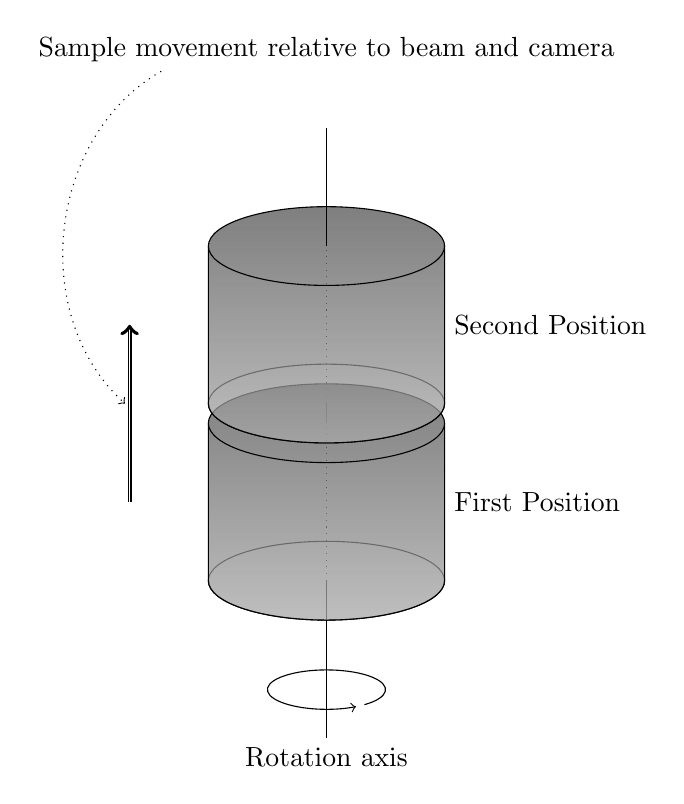
\begin{tikzpicture}%[ultra thick,scale=1]%,show background grid]
	%draw axes
		%\draw[ultra thick] (-10,0) -- (10,0);
		%\draw[ultra thick] (0,-10) -- (0,10);
		%\draw[ultra thick] (0,0) circle (.125);
	% rotation axis
		\draw[->] (0,-2) ++ (-50:.75) arc (-50:300:.75 and .25);
		\draw (0,-3) node [below] {Rotation axis} -- ++(0,2);
		\draw[dotted] (0,-1) -- ++(0,2);
		\draw (0,1) -- ++(0,0.25);
		\draw[dotted] (0,1.25) -- ++(0,2);
	% position 1
		\draw (0,-1) circle (1.5 and .5);
		\fill[shade,semitransparent] (-1.5,-1) arc (-180:0:1.5 and .5) -- ++(0,2) arc (0:180:1.5 and .5) -- cycle;
		\draw (-1.5,-1) arc (-180:0:1.5 and .5) -- ++(0,2) arc (0:180:1.5 and .5) -- cycle;		
		\draw (-1.5,1) arc (-180:0:1.5 and .5);
		\draw (1.5,0) node [right] {First Position};
	% position 2
		\draw (0,1.25) circle (1.5 and .5);
		\fill[shade,semitransparent] (-1.5,1.25) arc (-180:0:1.5 and .5) -- ++(0,2) arc (0:180:1.5 and .5) -- cycle;
		\draw (-1.5,1.25) arc (-180:0:1.5 and .5) -- ++(0,2) arc (0:180:1.5 and .5) -- cycle;		
		\draw (-1.5,3.25) arc (-180:0:1.5 and .5);
		\draw (1.5,2.25) node [right] {Second Position};
	% rotation axis on top
		\draw (0,3.25) -- ++(0,1.5);									
	% sample movement
		\draw[double,->] (-2.5,0) -- (-2.5,2.25) ;% node [text width=10cm,midway,left] {Sample movement relative to beam and camera};	
		% sample movement
		\node (movefrom) at (0,5.75) {Sample movement relative to beam and camera};
		\node (moveto) at (-2.5,1.125) {};
		\draw [->,dotted] (movefrom) to [bend right=54] (moveto);
\end{tikzpicture}
\end{preview}
\end{document}%
			\label{subfig:stacked-scan}%
		}%
	}% end of \makebox
	\caption[Covering the FOV of differently sized samples]{\subref{subfig:scanning-possibilities}: Covering the FOV of differently sized samples with one \SI{180}{\degree} scan (top), one \SI{360}{\degree} scan (center) or---in the case of the so called wide field scanning---with multiple subscans (three subscans, bottom) The filled red, green and blue segments mark the covered region of the sample for the respective positions. \subref{subfig:stacked-scan}: Increasing the vertical FOV with stacked scanning.
	}%
	\label{fig:scanning-possibilities}%
\end{figure*}

If we want to achieve tomographic scans covering a sample size which is bigger than what can be achieved with a \SI{360}{\degree}-scan, we have to move the sample in relation to the beam and camera. This can be done as shown in figure~\ref{subfig:scanning-possibilities}, where we obtain three subscans to be able to reconstruct a sample as big as three FOVs.

After correction with the dark and flat images, the projections of the single overlapping subscans are merged into one projection which covers the full FOV chosen by the user (see figure~\ref{fig:merge-proj}).

\cbstart
While covering the desired FOV, the projection images of each subscan need to overlap each other slightly to allow for an optimal stitching of the multiple projections into one big projection. Preliminary experiments \todo{do we need to write: ``results not shown''?} showed that an overlap of approximately 20 pixels allows for the calculation of the cutting line between the independent subscans with a precision of one pixel.
\cbend

As described by~\citet{Hintermueller2009}, the cutting line to remove the overlap is calculated using the mean squared difference between adjacent subscan images. Briefly, for each displacement $\xi_{i,j}$ of the images $i$ and $j$ the mean squared difference of the displacement $\delta^2(\xi_{i,j})$ is computed. This displacement measure provides a measure for the inequality of the two images within their overlapping parts. The local minimum of $\delta^2(\xi_{i,j})$ shows the effective displacement $\xi_{i,j}$ between the two adjacent images $i$ and $j$. For three subscans we calculate the effective displacement $\xi_{1,2}$ and $\xi_{2,3}$ and stitch all the images into one big projection image.

To fulfill the sampling theorem as defined in section~\ref{subsec:enhancing the field of view}, a different amount of projections ($N_{i}$) have been recorded for each subscan $i$---at the lateral positions we record more projections compared to the central position. A simple example is shown in figure~\ref{fig:projections}.

\cbstart
If we assume that we acquire only four projections for the central part of the sample, we need to acquire 16 projections for the lateral parts of the sample to be able to fulfill the sampling theorem\todo{Is there some ``formula'' we can cite instead of just saying it\ldots}.

We thus acquire a different amount of projections for the central and the lateral parts of the sample for the gold-standard case, thus our stitching algorithm has to selectively stitch projections from subscan 1 with several projections from subscan 2 and 3 to one projection covering the combined FOV.
\cbend

\cbstart
\begin{figure*}
	\centering
%	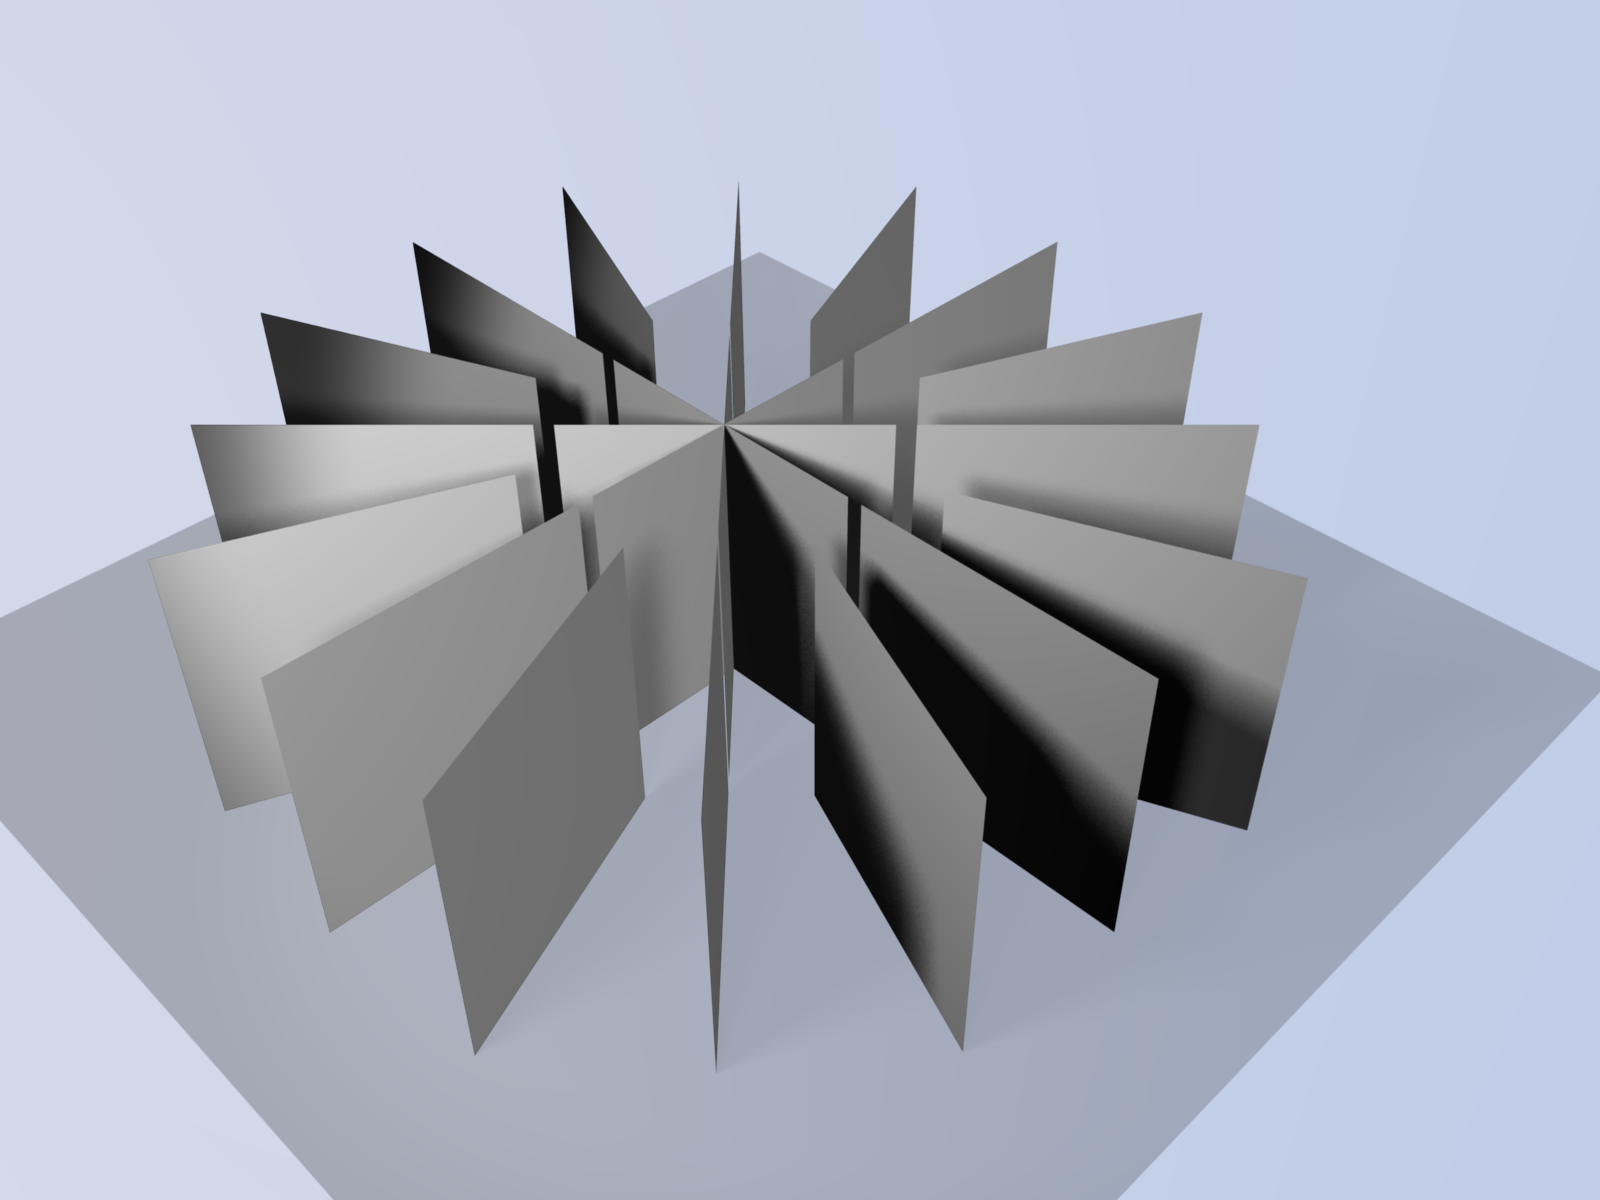
\includegraphics[width=\imsize]{img/projections}
	%\documentclass{article}
%\usepackage[demo]{graphicx}
%\usepackage{subfig}
%\usepackage{tikz}
%\usepackage{multirow}
%\usepackage{siunitx}
%\begin{document}
%\begin{figure}
%\centering
%%%%%%%%%%%%%%%%%%%%%%%%%%%%%
\def\radius{1}%
\def\gap{0.05}%
\begin{tikzpicture}[scale=.75]%
	\foreach \ang in {0,45,...,359}%
		{%
		\draw [ultra thick] (\ang:0) -- (\ang:\radius);%
		}%
	\foreach \ang in {0,45,...,359}%
		{%
		\draw [very thick, color=yellow, shorten >=0.25pt] (\ang:0) -- (\ang:\radius);%
		}%
	\foreach \ang in {0,22.5,...,179}%
		{%
		\draw [ultra thick] (\ang:\radius+\gap) -- (\ang:3*\radius+\gap);%
		\draw [very thick, color=magenta, shorten >=0.25pt,shorten <=0.25pt] (\ang:\radius+\gap) -- (\ang:3*\radius+\gap);%
		}%
	\foreach \ang in {180,202.5,...,359}%
		{%
		\draw [ultra thick] (\ang:\radius+\gap) -- (\ang:3*\radius+\gap);%		
		\draw [very thick, color=cyan, shorten >=0.25pt,shorten <=0.25pt] (\ang:\radius+\gap) -- (\ang:3*\radius+\gap);%
		}%
	\node [anchor=south west] at (-3.05,-3.05) {(a)};
\end{tikzpicture}
%%%%%%%%%%%%%%%%%%%%%%%%%%%%%	
%\caption{Projection Setup}
%\end{figure}
%\end{document}
	\caption{Setup with one central (green) and two lateral scans (red and blue, respectively). For demonstration purposes, the central scan has four projections and the lateral scans have eight projections each (all acquired over \SI{180}{\degree}. The colors of the three positions correspond to the colors shown in figure~\ref{subfig:scanning-possibilities}.}
	\label{fig:projections}
\end{figure*}
\cbend

Figure \ref{fig:amount of projections} shows how projections from the different subscans relate to each other. In this case we acquire 1500 projections for the central and two times 3000 projections for the two ring-scans to fully satisfy the sampling theorem. 

A simple strategy for designing the different protocols has been defined; to facilitate the merging of the projections from each subscan, the amount of projections from the inner to the outer subscans is always dividable by two.
\begin{equation}
	\frac{P_{outer}}{P_{inner}} \bmod 2 = 0
\label{eq:Modulo}
\end{equation}
This approach facilitates the merging of the different subscans in such a way that we can stitch several projections from the inner subscan with projections from the outer subscan as shown in figure~\ref{fig:amount of projections}. Equation~\ref{eq:Modulo} ensures that the stitching and---where applicable---interpolation of projections can be done in an efficient way. 

\begin{figure*}
	\centering
	%\documentclass{minimal}
%\usepackage[pdftex,active,tightpage]{preview}
%\usepackage{tikz}
%\begin{document}
%\begin{preview}
%\begin{center}
%%%%%%%%%%%%%%%%%%%%%%%%%%%%%	
	\def\radius{1}
	\def\shift{.3}
	\def\overlap{.075}
	\begin{tikzpicture}[scale=1.5]
		%% inner ring
		\draw (0,0) circle (\radius);
		\foreach \angle / \label in 
			{0,20,...,181}
			{
				\draw (\angle:-\radius) -- (\angle:\radius+\shift);
				\draw (\angle:\radius+1.618*\shift) node{\textsf{\label}};
			}
		\foreach \angle in 
			{0,2,...,180}
			{
				\draw (\angle:\radius-.5*\shift) -- (\angle:\radius+.5*\shift);
			}
		%% outer ring			
		\draw (0,0) circle (3*\radius);
		\foreach \angle / \label in 
			{0,20,...,719}
			{
				\draw (.5*\angle:\radius) -- (.5*\angle:3*\radius+\shift);
				\draw (.5*\angle:3*\radius+1.618*\shift) node{\textsf{\label}};
			}
		\foreach \angle in 
			{0,1,...,359}
			{
				\draw (\angle:3*\radius-.5*\shift) -- (\angle:3*\radius+.5*\shift);
			}
		\def\projangle{17}			
		%% RingScan 1
		\draw [ultra thick,color=red](\projangle:\radius-\overlap) -- (\projangle:3*\radius);
		\fill [color=red,nearly transparent] (1,0) -- (3,0) arc (0:180:3*\radius) -- (-1+\overlap,0) arc (180:0:\radius-\overlap);
		%% Central Scan
		\draw [ultra thick,color=green](\projangle+180+2:\radius+\overlap) -- (\projangle+2:\radius+\overlap);
		\fill [color=green,nearly transparent] (0,0) circle (\radius+\overlap);
		%% Ringscan 2
		\draw [ultra thick,color=blue](\projangle+180:3*\radius) -- (\projangle+180:\radius-\overlap);
		\fill [color=blue,nearly transparent] (1,0) -- (3,0) arc (0:-180:3*\radius) -- (-1+\overlap,0) arc (-180:0:\radius-\overlap);
	\end{tikzpicture}%
%%%%%%%%%%%%%%%%%%%%%%%%%%%%%	
%\end{center}
%\end{preview}
%\end{document}%
	\caption[Number of merged projections for one central- and two ring-scan.]{Number of merged projections for one central- and two ring-scan. We assume that we have obtained 1500 projections for the central scan and thus acquire two times 1500 projections for each of the lateral scans. This enables us to stitch the projections $P_{1_{283}}$ % XXX XXX 17*3000/180 XXX
    (red line) from subscan 1 (ring scan, red area), projection $P_{2_{142}}$ % XXX 17*1500/180 XXX
    (green line) from subscan 2 (central scan, green area) and projection $P_{3_{283}}$ % XXX 17*3000/180 XXX
    (blue line) of subscan 3 (ring scan, blue area) to one big projection $P_{merge_{283}}$ % XXX 17*3000/180 XXX
    which covers the full FOV. The areas of the three subscans overlap slightly as described above to account for variations in positioning. For illustration purposes we shifted the central projection (green) by \SI{2}{\degree}, or else the overlap between these particular projection would not be visible.}%
	\label{fig:amount of projections}%
\end{figure*}

\subsection{Wide Field Scanning}
\cbstart
A custom MATLAB-script (MATLAB\textregistered 7.6.0.321 (R2008a), The MathWorks, Inc.) has been written to enable the user to input the scanning parameters like desired FOV, detector width, desired overlap between the subscans, magnification and binning. According to these presets, the scripts calculated the necessary projections to fulfill the sampling theorem for the chosen FOV as a gold-standard and computes different protocols with reduced amount of projections. For all these scanning protocols a reconstruction is simulated using a Shepp-Logan phantom~\cite{Shepp1974} and the expected reconstruction quality is calculated using the difference image for each simulated reconstruction with the gold standard. This expected reconstruction quality is then plotted against the acquisition time. Such a plot is shown in figure~\ref{fig:2008c-qualityplot}. From this plot, the user selects a suitable protocol which balances the need for reconstruction quality and acquisition time.
\cbend

\begin{figure*}
	\centering
	%\documentclass{article}
%\usepackage{tikz,pgfplots}
%\usepackage[pdftex,active,tightpage]{preview}
%\begin{document}
%\begin{preview}
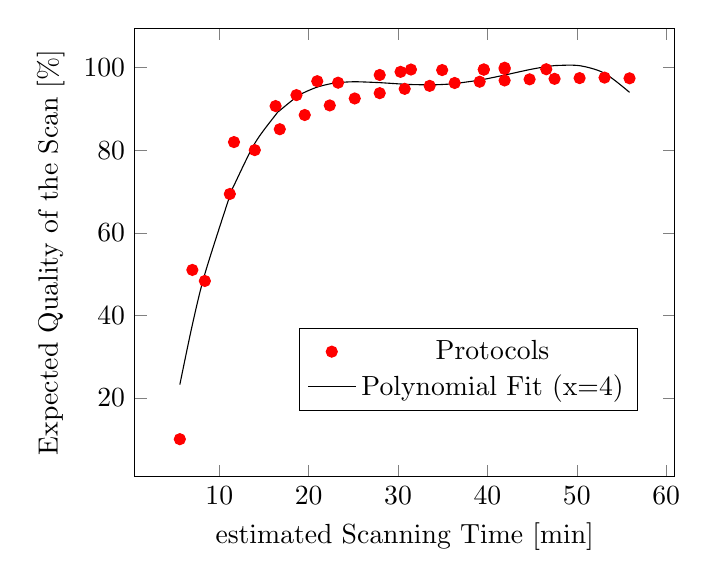
\begin{tikzpicture}
\begin{axis}[%
	xlabel={estimated Scanning Time [min]},%
	ylabel={Expected Quality of the Scan [\%]},%
	]

% Line plot
\addplot [ color = red, only marks, mark = *] 
coordinates{
 (5.5875,10) (6.98958,51.0063) (8.3875,48.3324) (11.1813,69.4075) (11.6458,81.985) (13.975,80.0399) (16.3021,90.7093) (16.7688,85.096) (18.6354,93.3621) (19.5625,88.5423) (20.9625,96.7319) (22.3625,90.8617) (23.2917,96.3704) (25.1563,92.5481) (27.9479,98.2413) (27.95,93.8354) (30.2813,98.9979) (30.7437,94.8773) (31.4438,99.5581) (33.5375,95.6051) (34.9375,99.4314) (36.3375,96.2983) (39.1313,96.6062) (39.5938,99.5875) (39.5958,99.5241) (41.925,100) (41.925,96.9138) (41.9271,99.6929) (44.7188,97.1848) (46.5833,99.6309) (47.5125,97.3067) (50.3125,97.4836) (53.1063,97.603) (55.9,97.4336)
};

% Line plot
\addplot [ smooth ] 
coordinates{
 (5.5875,23.213) (6.98958,37.7379) (8.3875,50.0404) (11.1813,68.9695) (11.6458,71.4736) (13.975,81.6837) (16.3021,88.5733) (16.7688,89.6234) (18.6354,92.9028) (19.5625,94.0559) (20.9625,95.3079) (22.3625,96.078) (23.2917,96.3777) (25.1563,96.6032) (27.9479,96.3862) (27.95,96.3859) (30.2813,96.0569) (30.7437,96.0006) (31.4438,95.9286) (33.5375,95.8484) (34.9375,95.9383) (36.3375,96.1591) (39.1313,96.986) (39.5938,97.167) (39.5958,97.1679) (41.925,98.211) (41.925,98.211) (41.9271,98.212) (44.7188,99.5426) (46.5833,100.268) (47.5125,100.516) (50.3125,100.492) (53.1063,98.6574) (55.9,94.0299)
};


\pgfplotsset{every axis legend/.append style={
at={(0.618,0.2)},
anchor=base}}

\legend{Protocols,Polynomial Fit (x=4)}%$p(x)=p_{1}x^{n}+p_{2}x^{n-1}+...+p_{n}x+p_{n+1}$}

\end{axis}
\end{tikzpicture}
%\end{preview}
%\end{document}%
	\caption[Quality-Plot of 34 calculated protocols]{Quality-Plot of 34 calculated protocols. The red dots show the expected quality of the different protocols, the black plot is a polynomial fit $p(x)$ with $n=4$ for $p(x)=p_{1}x^{n}+p_{2}x^{n-1}+\cdots+p_{n}x+p_{n+1}$. A subset of 19 protocols have been scanned. Details of these scans are shown in table~\ref{tab:projections} and are discussed in section~\ref{sec:Results}.}%
	\label{fig:2008c-qualityplot}%
\end{figure*}

After the user has chosen a suitable protocol (corresponding to one dot in figure~\ref{fig:2008c-qualityplot}), a preference file is written. This preference file is then subsequently parsed by a custom Python-script to interact with the EPICS-System (Experimental Physics and Industrial Control System, Argonne National Laboratory, Argonne, USA, \url{http://www.aps.anl.gov/epics/}), which itself is used to control the hardware of the TOMCAT beamline.

\subsubsection{Reduction of the acquisition time}
The proposed protocols are designed in such a way that the total scanning time---which scales with the total amount of recorded projections---can be greatly reduced. 

Depending on the input of the end-user, we were able to reduce the total acquisition time by \SI{86.8}{\percent} compared to the gold standard, as can be seen in table~\ref{tab:projections}. This table provides the details of the 19 different protocols we have scanned to examine and proof the simulation. This has been done to assess the artifacts which arise through the reduction of the amount of projections. Albeit the reduction in scanning time by \SI{86.8}{\percent} introduces artifacts in the reconstruction, an automated segmentation of the airways is still possible, as is shown in section~\ref{subsec:comparison}.
%\begin{table*}
%	\centering
%	\caption{Specification of different protocols and time used compared to gold standard}
%	\begin{tabular*}{\textwidth}{l@{\extracolsep\fill}ccccccccccccccccccc}
%		\toprule
%		Protocol 			& B & C & D & E & F & G & H\\
%		\midrule
%		Total Projections 	& 15732 & 13110 & 13110 & 10925 & 11799 & 9833 & 10488\\
%		Time [\%] 			& 100 & 83.33 & 83.33 & 69.44 & 75 & 62.5 & 66.67\\
%		\bottomrule
%	\end{tabular*}
%	\begin{tabular*}{\textwidth}{l@{\extracolsep\fill}ccccccccccccccccccc}
%		\toprule
%		Protocol 			& I & J & K & L & M & N \\
%		\midrule
%		Total Projections 	& 5436 & 8740 & 9177 & 7648 & 7866 & 6555 \\
%		Time [\%] 			& 34.7 & 55.6 & 58.3 & 48.6 & 50 & 41.7 \\
% 		\bottomrule
%	\end{tabular*}
%	\begin{tabular*}{\textwidth}{l@{\extracolsep\fill}ccccccccccccccccccc}
%		\toprule
%		Protocol 			& O & P & Q & R & S & T \\
%		\midrule
%		Total Projections 	& 6555 & 5244 & 4370 & 3933 & 2622 & 2185 \\
%		Time [\%] 			& 41.7 & 33.3 & 27.8 & 25 & 16.7 & 13.9 \\
%		\bottomrule
%	\end{tabular*}
%	\label{tab:projections}
%\end{table*}

\cbstart
\begin{table*}
	\centering
	\caption{Specification of different protocols and time used compared to gold standard. Protocol A corresponds to the Gold Standard, and would have been needed to cover the same FOV with 9 single scans with a detector width of 1024 pixels (plus an overlap of 100 pixels). This would result in a number of Projections $P=9*(1024+100)*\frac{\pi}{2}=15890$}
	\begin{tabular*}{\textwidth}{l@{\extracolsep\fill}ccccccc}
		\toprule
		Protocol & A & B & C & D & E & F & G \\
		\midrule
		Total Projections & 15890 & 15732 & 13110 & 13110 & 10925 & 11799 & 9833 \\
		Time [\%] &  100.0  &   99.0  &   82.5  &   82.5  &   68.8  &   74.3  &  61.9  \\
		\bottomrule
	\end{tabular*}
	\begin{tabular*}{\textwidth}{l@{\extracolsep\fill}ccccccc}
		\toprule
		Protocol & H & I & J & K & L & M & N \\
		\midrule
		Total Projections & 10488 & 8740 & 9177 & 7648 & 7866 & 6555 & 6555 \\
		Time [\%] & 66.0 & 55.0 & 57.8 & 48.1 & 49.5 & 41.3 & 41.3 \\
		\bottomrule
	\end{tabular*}
	\begin{tabular*}{\textwidth}{l@{\extracolsep\fill}cccccc}
		\toprule
		Protocol & O & P & Q & R & S & T \\
		\midrule
		Total Projections & 5463 & 5244 & 4370 & 3933 & 2622 & 2185 \\
		Time [\%] & 34.4 & 33.0 & 27.5 & 24.8 & 16.5 & 13.8 \\
		\bottomrule
	\end{tabular*}
	\label{tab:projections}
\end{table*}
\cbend

\cbstart
All subscans of each protocol have been scanned without any user intervention, except input of the sample name at the start of the batch-scan. All parameters such as sample-position in relation to the beam, rotation angles and amount of projections to obtain for the subscans have been set in a preference-file. For all 19 scanned protocols (B--T) the sample on the sample holder has not been touched, so that a direct comparison of the reconstructed slices is possible.

After acquisition of the three subscans per protocol, custom MATLAB functions read the parameters of the single subscans (e.g.\ sample name, amount of subscans, amount of dark and flat images) as well as the desired output-name and -suffix and performs all necessary calculations like loading of the correct projections from each subscan, normalizing, interpolation, cutline detection and correct stitching of the images into wide field projections. Exemplary results can be seen in figure~\ref{fig:subscans} and \ref{fig:merge-proj}. 

The merged projections were reconstructed into virtual tomography slices using an FFT-based gridrec algorithm~\cite{Dowd1999} on a 20-node server farm (five \SI{64}{\bit} Opteron machines with 4 cores and \SI{8}{\giga\byte} RAM each). The reconstructions result in an image stack covering a large sample volume of approximately 3000$\times$3000$\times$1024 pixels, a nine-fold increase from the standard volume of 1024$\times$1024$\times$1024 pixels for one single scan.
\cbend

The reconstructions used for the assessment of the image quality of the 19 different scanned protocols of the same sample show a three-fold (2.93\(\times\)) increase in FOV from 1024\(\times\)1024 pixels to 2996\(\times\)2996 pixels. As a proof of concept, we also scanned and reconstructed a lung sample with 5 subscans, which led to a roughly five-fold (4.74\(\times\)) increase in available FOV from 2048\(\times\)2048 pixels to 9703\(\times\)9703 pixels (see figure~\ref{fig:LungSlabSophie}).